\documentclass[12pt, a4paper]{article}
% \usepackage{mathtools}
\usepackage{graphicx}
\usepackage{amsthm}
\usepackage{hyperref}
\usepackage{amssymb}
\graphicspath{{images/}}

\hypersetup{
    colorlinks=true,
    linkcolor=blue,
    urlcolor=cyan
}

\title{Electric Potential Energy and Electric Potential}
\author{Franklin Chen}
\date{14 October 2024}

\theoremstyle{definition}
\newtheorem{definition}{Definition}

\begin{document}
\maketitle
\newpage
% comment

\tableofcontents

\section{Electric Potential Energy}
Similar to gravity, the electrostatic force ($F = k|q_1 q_2|/r^2$) is conservative, and thus has a corresponding potential energy.
Recall that the work done by the gravitational force when a ball falls from a height of $h_I$ to a height of $h_F$ is the difference between the two gravitational potential energies:

\[W_{I \to F} = {\textrm{GPE}}_I - {\textrm{GPE}}_F\]

Analgously, consider a charged particle (charge = $+q_0$) at some point I between two positively and negatively charged points.
Because of the plate charges, the electric field $\vec{E}$ exerts an electrostatic force $\vec{F} = q_0\vec{E}$ directed towards the negative plate.
The work done by the electric force moving the charged particle from point I to point F ($W_{I \to F}$) is equal to the difference in electric potential energies at the two points:

\[W_{I \to F} = {\textrm{EPE}}_I - {\textrm{EPE}}_F\]

Because the electrostatic force is conservative, the work $W_{I \to F}$ is a function purely of the initial and final states, regardless of the path taken.

\section{Electric Potential}
Because the force (and thus the work) exerted on a charged particle is dependent on the magnitude of the charge, it is useful to express the work on a \textbf{per-unit-charge basis}:

\[\frac{W_{I \to F}}{q_0} = \frac{{\textrm{EPE}}_I}{q_0} - \frac{{\textrm{EPE}}_F}{q_0}\]

The quantity $\frac{\textrm{EPE}}{q_0}$ is known as the \textbf{electric potential}:

\begin{definition}[Electric Potential, Potential]
    The electric potential V at a given point is the EPE of a small test charge $q_0$ at that point divided by the charge itself:
    (SI units joule/coloumb = volts (V))
    \[V = \frac{\textrm{EPE}}{q_0}\]
\end{definition}

Electric potential is often written as the final minus the initial, leading to the following convention:

\[\Delta V = \frac{\Delta \textrm{EPE}}{q_0} = \frac{-W_{I \to F}}{q_0}\]

The potential difference between two points is measured in volts, and is often referred to as \textit{voltage}.
This is the case for batteries, where the voltage between the positive and negative terminals (indirectly) indicate the rate at which electrons travel from the negative terminal to the positive one.

One \textbf{electron volts} (eV) is the magnitude of the amount by which the potential energy of an electron changes when it moves through a potential difference of one volt.
Specifically, $1 \textrm{eV} = |q_0 \Delta V| = |(-1.60 \times 10^{-19} \textrm{C}) \times (1.00 \textrm{V})| = 1.60 \times 10^{-19} \textrm{J}$.

Remember that EPE is an energy as well, and also follow the Law of Conservation of Energy.

It should be fairly obvious that positive charges will accelerate from regions of high electric potential (near the positive plate) to regions of lower electric potential (near the negative plate), and vice versa.

\section{Electric Potential created by Point Charges}
A point charge $+q$ creates an electric potential in the same way as a plate does.
Consider a test charge $+q_0$ some distance $r_I$ away from the point charge.
From Coloumb's law, the magnitude of force acting on the test charge is $F = kqq_0/r^2$, where we assume that $q_0$ and $q$ are positive.
The work done by the electric force as the test charge moves to some further distance $r_F$ can be calculated as follows:

\[W_{I \to F} = \int_{r_I}^{r_F} F(r)dr = \int_{r_I}^{r_F} \frac{kqq_0}{r^2}dr = kqq_0 (-\frac{1}{r} \Big|_{r_I}^{r_F}) = \frac{kqq_0}{r_I} - \frac{kqq_0}{r_F}\]

Thus, the voltage between I and F can be found:

\[\Delta V = \frac{-W_{I \to F}}{q_0} = \frac{kq}{r_F} - \frac{kq}{r_I}\]

As $\lim_{r_F \to \infty}$, we can see $V_I = kq/r_I$. This is the \textbf{potential of a point charge}, often written $V = kq/r$.

The V in this equation does not directly refer to the potential, but rather \textit{the amount by which the potential at a distance r from a point charge differs vs. if the charge wasn't there (at infinity).}
Note that this equation also includes the sign of the charge; negative potentials indicate that the potential is decreased below the "zero reference value."

Given many point charges, the electric potential at any point is the sum of the potentials of each point charge.

\newpage

\section{Equipotential Surfaces}
\begin{figure}
    \centering
    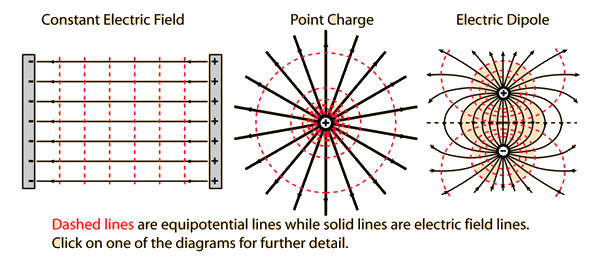
\includegraphics[width=1\textwidth]{equiv.jpg}
    \caption{Visualizations of the equipotential and electric field lines on a parallel plate capacitor, a single point charge, and an electric dipole.}
    \label{fig:equiv}
\end{figure}

\begin{definition}[Equipotential Surface]
    An imaginary surface on which the electric potential is the same everywhere.
    There are an infinite number of such surfaces.
\end{definition}

The relation $V_B - V_A = -W_{A \rightarrow B}/q_0$ suggests that if $V_A = V_B$, as on a equipotential surface, no work is done by the electric force.
Work is only done when a charge moves between equipotential surfaces.

For single point charges, the equation $V=kq/r$ suggests that the equipotential surfaces for a single point charges are spheres centered at the charge (constant r).

\textit{Electric field lines are everywhere perpendicular to all equipotential surfaces.}
Electric field lines give the direction of the electric field, outward for a positive test charge.
If electric field lines weren't perpendicular, then it would be able to project a parallel component of the electric field onto the equipotential field.
This suggests that a particle moving along that projected field would experience work (due to the electric field) and thus change potential, violating our assumption of a equipotential surface. 
\textit{This is true for all such equipotential surfaces; even those with multiple charges!}

In Figure \ref{fig:equiv}, the equipotential surfaces are shown in dashed red, while the electric field lines are shown as solid black.
It can be observed that at all intersection points between the two are always perpendicular.

There is a quantative way to relate the electric field and the equipotential surfaces.
Consider the parallel plate capacitor in Figure \ref{fig:equiv}.
It has been shown previously that the electric field between the plates is perpendicular to the plates and is constant everywhere.
Similarly, it can be shown that the equipotential surfaces must be planes parallel to the capacitor plates (to be perpendicular to the electric field lines).\\

Denote a point on the positive plate p and another point on the negative plate n.
As shown previously, the potential difference between the plates is equal to

\[V_p - V_n = \frac{W_{p \rightarrow n}}{q_0}\]

Consider a test charge $+q_0$ moving from some point p to point n.
From the definition of work:

\[W_{p \rightarrow n} = F\Delta s = q_0E\Delta s\]

Substituting this into the equation for the potential difference:

\[V_p - V_n = \frac{q_0E\Delta s}{q_0} = E\Delta s \Rightarrow E = \frac{V_p - V_n}{\Delta s}\]

The quantity $\Delta V / \Delta s$ is known as the \textbf{potential gradient} (units volts/meter).
The idea of the potential gradient can be applied to any scenario.

When applying the idea to parallel plate capacitors specifically, this is idea is often written as $E=V/d$, where $V = \max(V_p, V_n) - \min(V_p, V_n)$, and $d = s_p - s_n$.

\section{Capacitors and Dielectrics}

\begin{definition}[Capacitor]
    Two conductors (plates) of any shape placed near one another, but not touching.
\end{definition}

Capacitors store electric charge.
Each plate carries a charge of \textit{the same magnitude}: one negative, one positive.
Because of the different sign, the positive capacitor plate has a greater electric potential vs the negative plate.
This difference is denoted V.
V is proportional to the magnitude of the charge q. This is often expressed as

\[q = CV\]

The proportionality constant C is known as \textbf{capacitance}, and has SI units columb/volt = farad (F).

The region between the conductors or plates is often filled with an electrically insulating material, known as a \textbf{dielectric}.
The charge on the plate causes dipole moments in the dielectric, making the ends of the dielectric slightly positive and negative respectively.
Because of the surface charges in the diaelectric, a reduced number of the electric field lines generated by the charges on the plates are able to pass through the dielectric.
Some of the electric field lines on the ngative surfaces charges and begins on the other side of the dielectric.

As such, the electric field inside the dielectric is much less strong vs. the electric field inside the empty capacitor (assuming constant charge).
This reduction in electric field is described by the \textbf{dielectric constant} ($\kappa$).
If the capacitor has field magnitude $E_0$ before the dielectric and $E$ afterwards:

\[\kappa = \frac{E_0}{E}\]

The value of the dielectric constant depends on the nature of the dielectric material. \\

For parallel capacitors, the relation $E = V/d$ can be used (along with the relation $E_0 = q/(\epsilon_0 A)$: when was this equation discussed???)

\[E = \frac{E_0}{\kappa} = \frac{V}{d} \Rightarrow q = (\frac{\kappa \epsilon_0 A}{d})V = CV \Rightarrow C = \frac{\kappa \epsilon_0 A}{d}\]

This can be used to show that the capacitance with the diaelectric present is raised by a factor of $\kappa$ over the capacitance without it ($\kappa_{vaccum} = 1$).

\subsection{Energy Storage in a Capacitor}

When a capacitor is charged, it also stores energy.
For example, consider a battery doing work as it transfers an increment of charge from one plate to the other.
$W = qV$ may be applied, but as each increment of charge is moved, the potential difference increases, thus increasing the work per subsequent charge.

It can be shown that the total work done is the product of the total charge transfered q, and the average potential difference $\bar{V} = \frac{1}{2}V$:
Using this and $q = CV$, the expression of energy stored in a capacitor U can be expressed in several ways:

\[U = \frac{1}{2}qV = \frac{1}{2}CV^2 = \frac{q^2}{2C}\]

If we are considering a parallel plate capacitor, we can additionally use the equations $V = Ed$ and $C = \kappa \epsilon_0 A/d$:

\[U = \frac{1}{2}CV^2 = \frac{1}{2}(\frac{\kappa \epsilon_0 A}{d})(Ed)^2 = \kappa \epsilon_0 AdE^2\]

The quantity $Ad$ is equal to the volume between the plates, so the energy per unit volume, or the \textit{energy density} u is

\[u = \kappa \epsilon_0 E^2\]

It can be shown that this expression is valid for any electric field strength, not just that between the plates of a capacitor.




\end{document}